% autosearch_figures.tex — A4 Formatted Figures (4 Pages)
% Compile with: pdflatex autosearch_figures.tex (x2 for pgfplots)
\documentclass[a4paper,11pt]{article}
\usepackage[utf8]{inputenc}
\usepackage[margin=2cm]{geometry} 
\usepackage{tikz}
\usepackage{pgfplots}
\usepackage{algorithm2e}
\usepackage{amsmath,amssymb}
\usepackage{xcolor}

\usetikzlibrary{
  shapes.geometric,
  arrows.meta,
  positioning,
  fit,
  backgrounds,
  calc,
  decorations.pathreplacing
}
\pgfplotsset{compat=1.18}

% Colour palette
\definecolor{keepgreen}{HTML}{2E8B57}
\definecolor{discardred}{HTML}{CD3333}
\definecolor{llmpurple}{HTML}{7B68EE}
\definecolor{trainblue}{HTML}{4682B4}
\definecolor{gitgray}{HTML}{555555}
\definecolor{bglight}{HTML}{F5F5F5}
\definecolor{phasebg}{HTML}{E8E8F0}
\definecolor{bugred}{HTML}{FF4444}
\definecolor{contextgold}{HTML}{DAA520}

\begin{document}

\pagestyle{empty}

% ================================================================
% PAGE 1: FIGURE 1 — Protocol Diagram (Flowchart v1)
% ================================================================
\vspace*{\fill}
\begin{center}
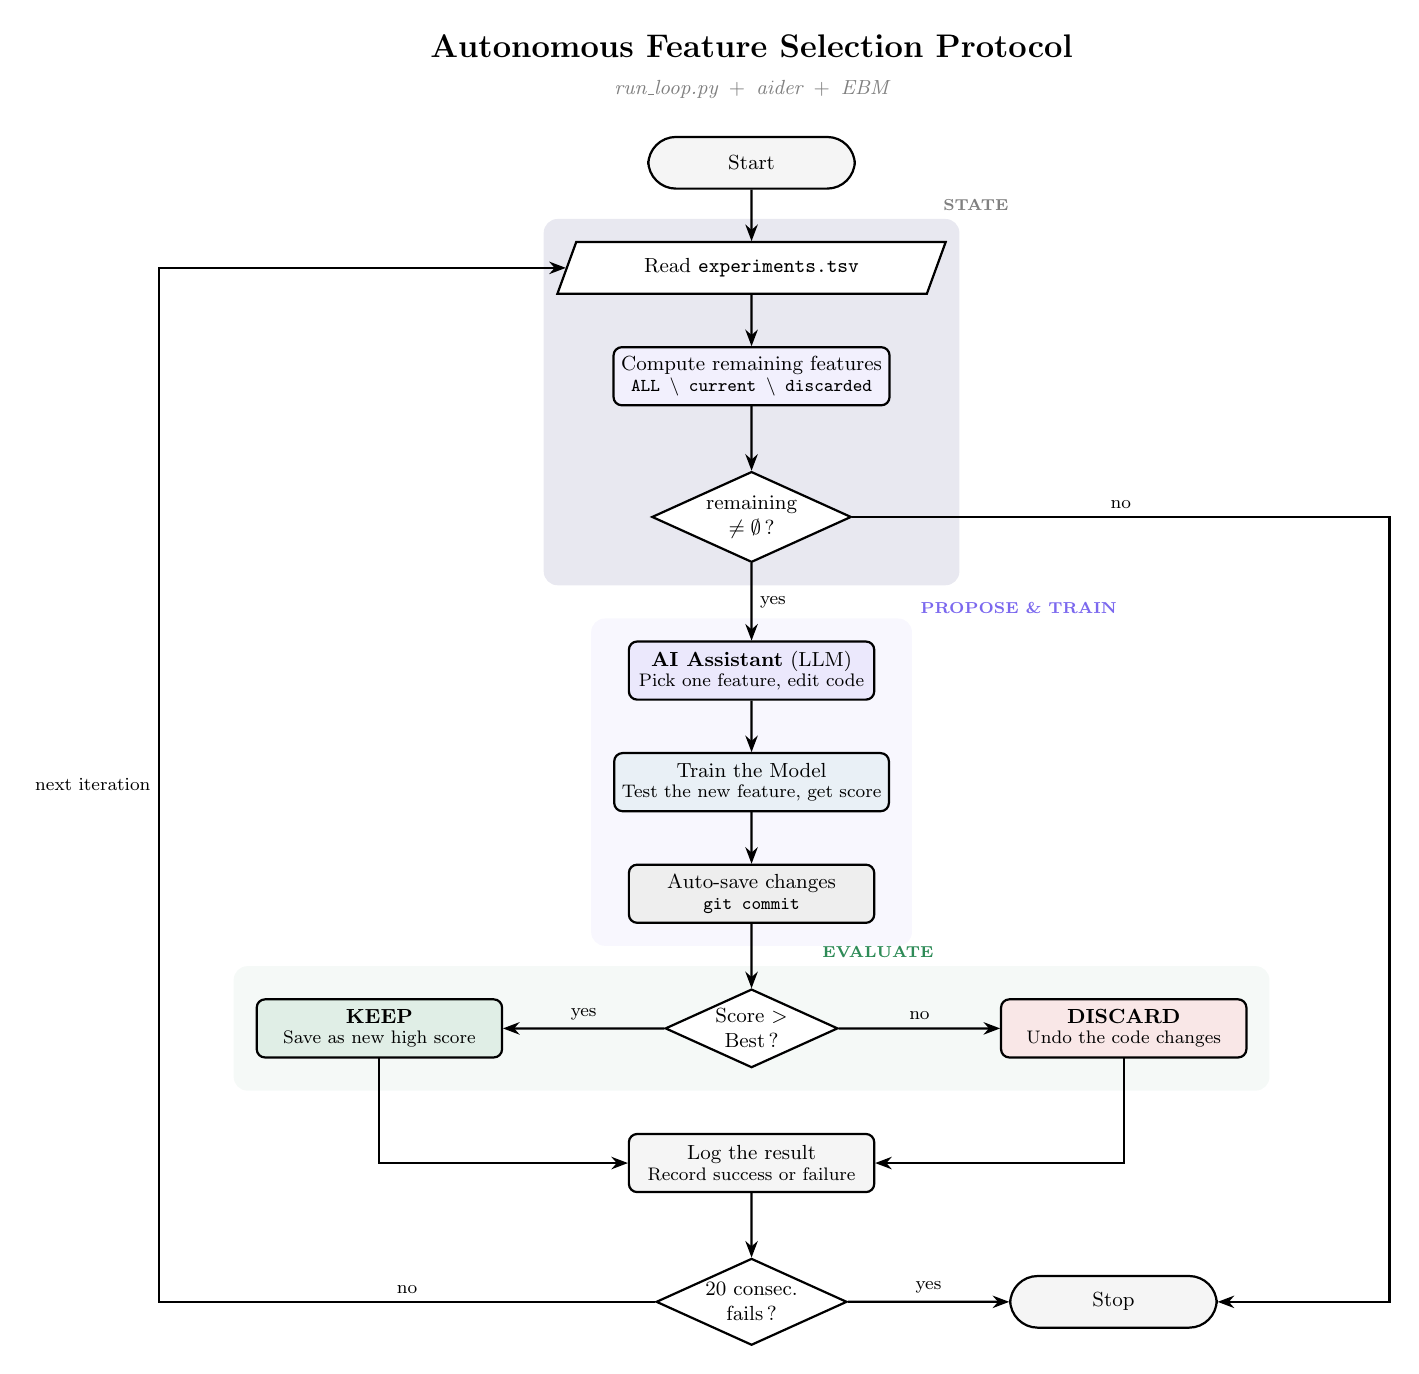
\begin{tikzpicture}[
    scale=0.82, transform shape, % Native TikZ scaling (Safe for A4)
    node distance=1.2cm and 2.5cm,
    every node/.style={font=\small, align=center},
    process/.style={
      rectangle, draw, rounded corners=3pt,
      minimum width=3.8cm, minimum height=0.9cm,
      fill=white, thick
    },
    decision/.style={
      diamond, draw, thick,
      minimum width=2.2cm, minimum height=1.2cm,
      inner sep=1pt, fill=white,
      aspect=2.2
    },
    startstop/.style={
      rectangle, draw, rounded corners=10pt,
      minimum width=3.2cm, minimum height=0.8cm,
      fill=bglight, thick
    },
    io/.style={
      trapezium, draw, thick,
      trapezium left angle=70, trapezium right angle=110,
      minimum width=3cm, minimum height=0.8cm,
      fill=white
    },
    arrow/.style={-{Stealth[length=6pt]}, thick},
    dasharrow/.style={-{Stealth[length=5pt]}, thick, dashed, gray},
  ]

  % --- Title ---
  \node[font=\Large\bfseries, anchor=south] at (0, 11.5)
    {Autonomous Feature Selection Protocol};
  \node[font=\small\itshape, anchor=north, text=gray] at (0, 11.4)
    {run\_loop.py $\,+\,$ aider $\,+\,$ EBM};

  % --- Nodes ---
  \node[startstop] (start) at (0, 10) {Start};
  \node[io, below=0.8cm of start] (readstate)
    {Read \texttt{experiments.tsv}};
  \node[process, below=0.8cm of readstate, fill=llmpurple!10] (remaining)
    {Compute remaining features\\[-2pt]
     {\footnotesize \texttt{ALL $\setminus$ current $\setminus$ discarded}}};
  \node[decision, below=1cm of remaining] (anyleft)
    {remaining\\$\neq \emptyset$\,?};
  \node[process, below=1.2cm of anyleft, fill=llmpurple!15] (llm)
    {\textbf{AI Assistant} (LLM)\\[-2pt]
     {\footnotesize Pick one feature, edit code}};
  \node[process, below=0.8cm of llm, fill=trainblue!12] (train)
    {Train the Model\\[-2pt]
     {\footnotesize Test the new feature, get score}};
  \node[process, below=0.8cm of train, fill=gitgray!10] (commit)
    {Auto-save changes\\[-2pt]
     {\footnotesize \texttt{git commit}}};
  \node[decision, below=1cm of commit] (improved)
    {Score $>$\\Best\,?};

  % Keep branch (left)
  \node[process, left=2.5cm of improved, fill=keepgreen!15] (keep)
    {\textbf{KEEP}\\[-2pt]
     {\footnotesize Save as new high score}};
  % Discard branch (right)
  \node[process, right=2.5cm of improved, fill=discardred!12] (discard)
    {\textbf{DISCARD}\\[-2pt]
     {\footnotesize Undo the code changes}};

  \node[process, below=1cm of improved, fill=bglight] (log)
    {Log the result\\[-2pt]
     {\footnotesize Record success or failure}};
  \node[decision, below=1cm of log] (stopcheck)
    {20 consec.\\fails\,?};

  \node[startstop, right=2.5cm of stopcheck] (stop) {Stop};

  % --- Safe Routing Coordinates for Loop Arrows ---
  \coordinate (rightRoute) at ($ (discard.east) + (2.2cm, 0) $);
  \coordinate (leftRoute) at ($ (keep.west) - (1.5cm, 0) $);

  % --- Arrows ---
  \draw[arrow] (start) -- (readstate);
  \draw[arrow] (readstate) -- (remaining);
  \draw[arrow] (remaining) -- (anyleft);
  \draw[arrow] (anyleft) -- node[right, font=\footnotesize] {yes} (llm);
  
  \draw[arrow] (anyleft.east) -- node[above, font=\footnotesize] {no} 
    (anyleft.east -| rightRoute) -- 
    (stop.east -| rightRoute) -- (stop.east);
    
  \draw[arrow] (llm) -- (train);
  \draw[arrow] (train) -- (commit);
  \draw[arrow] (commit) -- (improved);

  \draw[arrow] (improved.west) -- node[above, font=\footnotesize] {yes} (keep.east);
  \draw[arrow] (improved.east) -- node[above, font=\footnotesize] {no} (discard.west);

  \draw[arrow] (keep.south) |- (log);
  \draw[arrow] (discard.south) |- (log);

  \draw[arrow] (log) -- (stopcheck);
  \draw[arrow] (stopcheck.east) -- node[above, font=\footnotesize] {yes} (stop.west);
  
  \draw[arrow] (stopcheck.west) -- node[above, font=\footnotesize] {no} 
    (stopcheck.west -| leftRoute) -- 
    node[left, font=\footnotesize] {next iteration} 
    (readstate.west -| leftRoute) -- (readstate.west);

  % --- Phase labels (right side) ---
  \begin{scope}[on background layer]
    \node[fit=(readstate)(remaining)(anyleft),
      fill=phasebg, rounded corners=5pt, inner sep=8pt,
      label={[font=\scriptsize\bfseries, text=gray]above right:STATE}] {};
    \node[fit=(llm)(train)(commit),
      fill=llmpurple!5, rounded corners=5pt, inner sep=8pt,
      label={[font=\scriptsize\bfseries, text=llmpurple]above right:PROPOSE \& TRAIN}] {};
    \node[fit=(improved)(keep)(discard),
      fill=keepgreen!5, rounded corners=5pt, inner sep=8pt,
      label={[font=\scriptsize\bfseries, text=keepgreen]above right:EVALUATE}] {};
  \end{scope}
\end{tikzpicture}
\end{center}
\vspace*{\fill}

\newpage
% ================================================================
% PAGE 2: FIGURE 2 — Pseudocode (Layperson Friendly)
% ================================================================
\vspace*{\fill}
\begin{center}
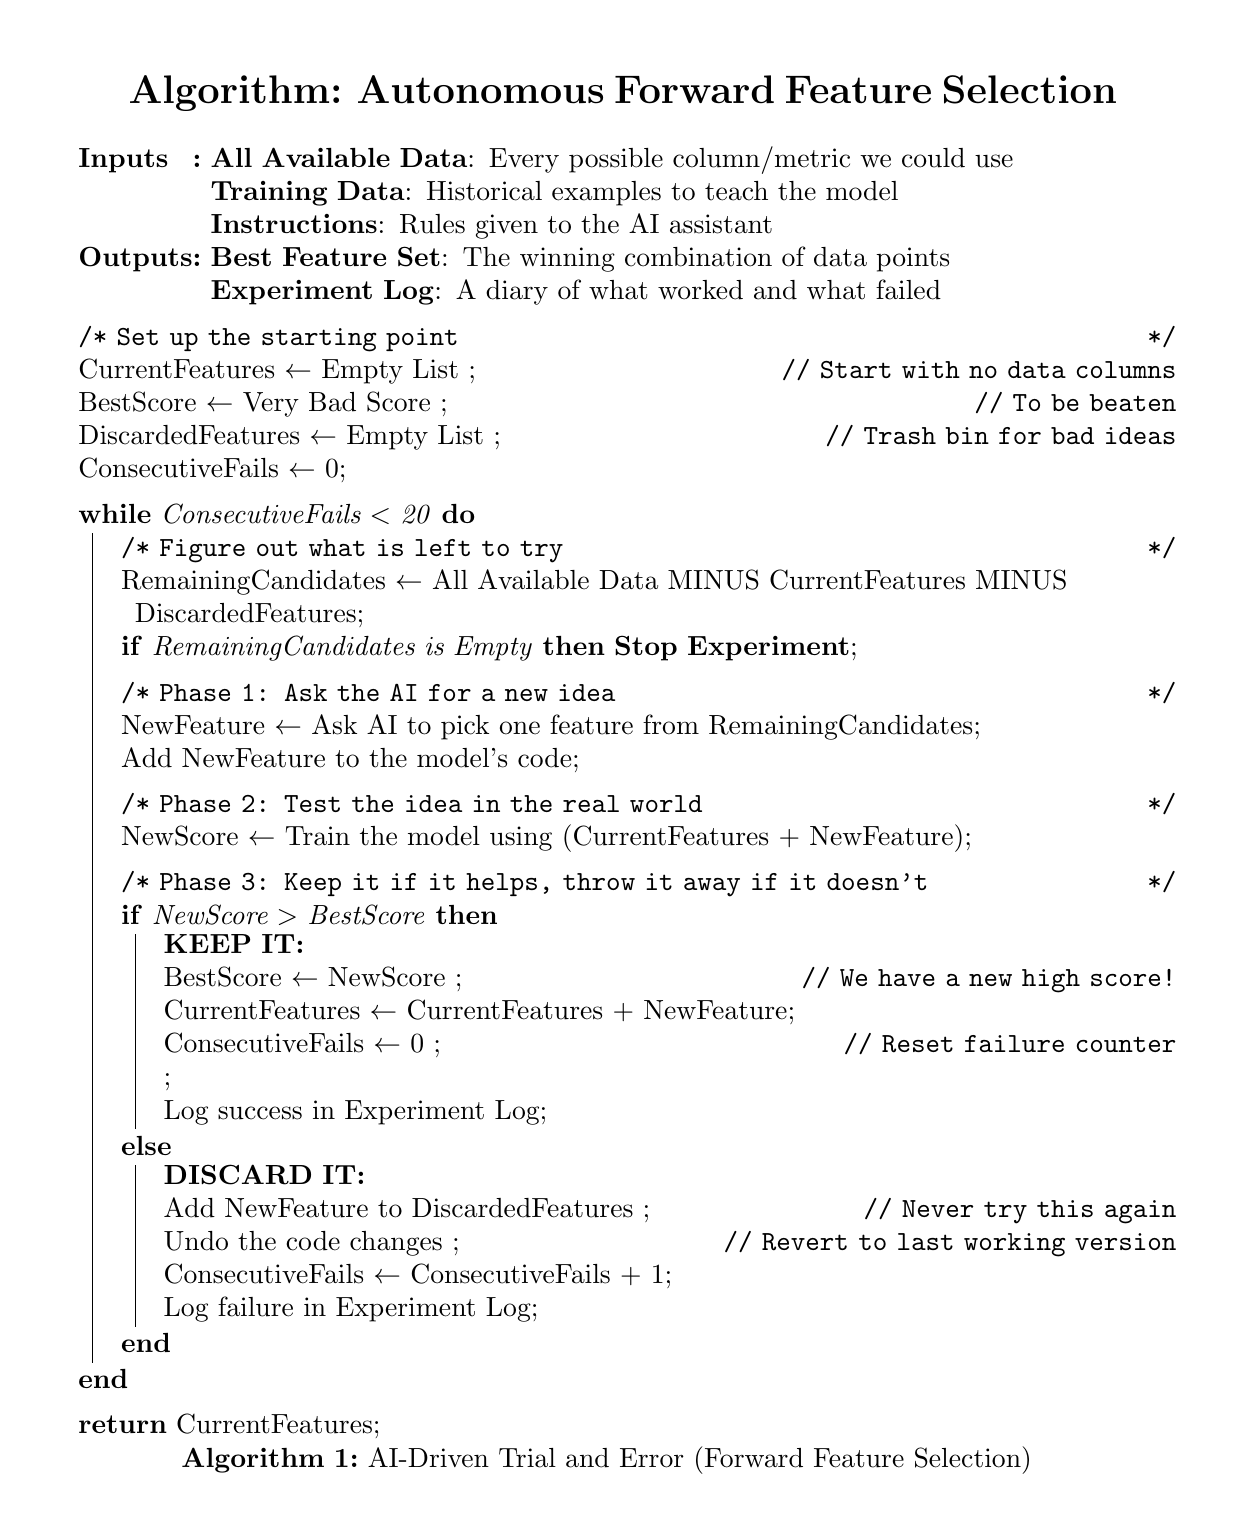
\begin{tikzpicture}
  \node[anchor=center, text width=15cm] at (0,0) {
    \begin{minipage}{15cm}
    \vspace{0.5cm}
    \centering
    {\Large\bfseries Algorithm: Autonomous Forward Feature Selection}
    \vspace{0.3cm}

    \begin{algorithm}[H]
      \SetAlgoLined
      \SetKwInOut{Input}{Inputs}
      \SetKwInOut{Output}{Outputs}

      \Input{%
        \textbf{All Available Data}: Every possible column/metric we could use\\
        \textbf{Training Data}: Historical examples to teach the model\\
        \textbf{Instructions}: Rules given to the AI assistant
      }
      \Output{%
        \textbf{Best Feature Set}: The winning combination of data points\\
        \textbf{Experiment Log}: A diary of what worked and what failed
      }
      \BlankLine

      \tcc{Set up the starting point}
      CurrentFeatures $\leftarrow$ Empty List \tcp*{Start with no data columns}
      BestScore $\leftarrow$ Very Bad Score \tcp*{To be beaten}
      DiscardedFeatures $\leftarrow$ Empty List \tcp*{Trash bin for bad ideas}
      ConsecutiveFails $\leftarrow$ 0\;

      \BlankLine
      \While{ConsecutiveFails $<$ 20}{
        \tcc{Figure out what is left to try}
        RemainingCandidates $\leftarrow$ All Available Data MINUS CurrentFeatures MINUS DiscardedFeatures\;
        \lIf{RemainingCandidates is Empty}{\textbf{Stop Experiment}}
        \BlankLine

        \tcc{Phase 1: Ask the AI for a new idea}
        NewFeature $\leftarrow$ Ask AI to pick one feature from RemainingCandidates\;
        Add NewFeature to the model's code\;

        \BlankLine
        \tcc{Phase 2: Test the idea in the real world}
        NewScore $\leftarrow$ Train the model using (CurrentFeatures + NewFeature)\;

        \BlankLine
        \tcc{Phase 3: Keep it if it helps, throw it away if it doesn't}
        \eIf{NewScore $>$ BestScore}{
          \textbf{KEEP IT:}\\
          BestScore $\leftarrow$ NewScore \tcp*{We have a new high score!}
          CurrentFeatures $\leftarrow$ CurrentFeatures + NewFeature\;
          ConsecutiveFails $\leftarrow$ 0 \tcp*{Reset failure counter}\;
          Log success in Experiment Log\;
        }{
          \textbf{DISCARD IT:}\\
          Add NewFeature to DiscardedFeatures \tcp*{Never try this again}
          Undo the code changes \tcp*{Revert to last working version}
          ConsecutiveFails $\leftarrow$ ConsecutiveFails + 1\;
          Log failure in Experiment Log\;
        }
      }
      \BlankLine
      \Return CurrentFeatures\;

      \caption{AI-Driven Trial and Error (Forward Feature Selection)}
    \end{algorithm}
    \end{minipage}
  };
\end{tikzpicture}
\end{center}
\vspace*{\fill}

\newpage
% ================================================================
% PAGE 3: FIGURE 3 — Experiment Evolution Graph (Dual Axis)
% ================================================================
\vspace*{\fill}
\begin{center}
\begin{tikzpicture}
  % MAIN AXIS (Left Side - Scientific)
  \begin{axis}[
    title={\textbf{Model Performance Evolution}},
    title style={font=\Large},
    width=0.78\textwidth, 
    height=11.5cm,
    xlabel={Experiment \#},
    ylabel={Scientific Score (neg. log-loss, higher $=$ better)},
    xmin=0, xmax=58,
    ymin=-0.55, ymax=-0.25, 
    grid=major,
    grid style={gray!20},
    legend pos=south east,
    legend style={font=\small, fill=white, fill opacity=0.9, draw=gray!50},
    tick label style={font=\small},
    label style={font=\normalsize},
    every node near coord/.append style={font=\tiny, rotate=70, anchor=west},
    clip=false,
    axis y line*=left,
  ]

    % --- Keep points ---
    \addplot[
      only marks, mark=*, mark size=2.5pt,
      color=keepgreen, fill=keepgreen,
    ] coordinates {
      (1,-0.481900) (2,-0.424476) (4,-0.425256) (6,-0.425993) (8,-0.425884) (9,-0.424644)
      (10,-0.424145) (11,-0.423191) (12,-0.322244) (13,-0.310729) (14,-0.310585) (15,-0.304235)
      (17,-0.305019) (18,-0.304037) (20,-0.307497) (22,-0.308363) (23,-0.301269) (24,-0.300531)
      (25,-0.300142) (26,-0.298393) (27,-0.298049) (28,-0.297776) (29,-0.297071) (30,-0.294875)
      (31,-0.294821) (33,-0.295992) (34,-0.295108) (35,-0.294700) (36,-0.294367) (37,-0.293819)
      (38,-0.293323) (39,-0.290408) (40,-0.288227) (42,-0.289002) (43,-0.284555) (44,-0.282259)
      (46,-0.281416) (48,-0.281829) (50,-0.282599) (52,-0.283061) (54,-0.284236) (55,-0.282977)
      (56,-0.282509)
    };
    \addlegendentry{Keep (Improved)}

    % --- Discard points ---
    \addplot[
      only marks, mark=x, mark size=3pt,
      color=discardred, thick,
    ] coordinates {
      (3,-0.425860) (5,-0.425841) (7,-0.426578) (16,-0.305333) (19,-0.307497) (21,-0.308363)
      (32,-0.295992) (41,-0.288644) (45,-0.282310) (47,-0.281829) (49,-0.282599) (51,-0.283061)
      (53,-0.284354)
    };
    \addlegendentry{Discard (Failed)}

    % --- True monotonic best ---
    \addplot[
      no marks, thick, dashed, color=trainblue, opacity=0.7,
    ] coordinates {
      (1,-0.481900) (2,-0.424476) (12,-0.424476) (12,-0.322244) (13,-0.310729) (14,-0.310585)
      (15,-0.304235) (18,-0.304235) (18,-0.304037) (23,-0.304037) (23,-0.301269) (24,-0.300531)
      (25,-0.300142) (26,-0.298393) (27,-0.298049) (28,-0.297776) (29,-0.297071) (30,-0.294875)
      (31,-0.294821) (35,-0.294821) (35,-0.294700) (36,-0.294367) (37,-0.293819) (38,-0.293323)
      (39,-0.290408) (40,-0.288227) (44,-0.288227) (44,-0.282259) (46,-0.282259) (46,-0.281416)
      (56,-0.281416)
    };
    \addlegendentry{True Best Trend}

    % --- Key annotations ---
    \draw[decorate, decoration={brace, amplitude=5pt, mirror}, thick, gray]
      (axis cs:1,-0.52) -- (axis cs:11,-0.52)
      node[midway, below=5pt, font=\scriptsize\itshape, text=gray] {Static data points added};

    % Phase: precipitation onset
    \draw[-{Stealth}, thick, trainblue]
      (axis cs:12,-0.35) -- (axis cs:12,-0.325)
      node[above=2pt, font=\scriptsize\bfseries, text=trainblue] {1-day precip added};

    \draw[decorate, decoration={brace, amplitude=5pt, mirror}, thick, gray]
      (axis cs:12,-0.52) -- (axis cs:56,-0.52)
      node[midway, below=5pt, font=\scriptsize\itshape, text=gray]
      {Dynamic data points tested};

    % Bug annotation: discard-then-keep pairs
    \draw[thick, bugred, opacity=0.4] (axis cs:19,-0.307497) circle (6pt);
    \draw[thick, bugred, opacity=0.4] (axis cs:21,-0.308363) circle (6pt);
    \draw[thick, bugred, opacity=0.4] (axis cs:32,-0.295992) circle (6pt);
    \draw[thick, bugred, opacity=0.4] (axis cs:47,-0.281829) circle (6pt);
    \draw[thick, bugred, opacity=0.4] (axis cs:49,-0.282599) circle (6pt);
    \draw[thick, bugred, opacity=0.4] (axis cs:51,-0.283061) circle (6pt);
    
    \node[font=\scriptsize, text=bugred, anchor=west] at (axis cs:52.5,-0.308)
      {\textbf{Code Bug}:};
    \node[font=\scriptsize, text=bugred, anchor=west] at (axis cs:52.5,-0.315)
      {(Rejected item re-accepted)};
    \draw[-{Stealth}, bugred, thick] (axis cs:52.3,-0.306) -- (axis cs:21.5,-0.3075);

    % Feature count axis
    \node[font=\tiny, text=gray, anchor=south] at (axis cs:1,-0.265) {1 item};
    \node[font=\tiny, text=gray, anchor=south] at (axis cs:11,-0.265) {8 items};
    \node[font=\tiny, text=gray, anchor=south] at (axis cs:15,-0.265) {12 items};
    \node[font=\tiny, text=gray, anchor=south] at (axis cs:31,-0.265) {25 items};
    \node[font=\tiny, text=gray, anchor=south] at (axis cs:40,-0.265) {33 items};
    \node[font=\tiny, text=gray, anchor=south] at (axis cs:56,-0.265) {43 items};

  \end{axis}

  % SECONDARY AXIS (Right Side - Layperson Friendly)
  \begin{axis}[
    width=0.78\textwidth, 
    height=11.5cm,
    xmin=0, xmax=58,
    ymin=-0.55, ymax=-0.25, 
    hide x axis,
    axis y line*=right,
    ylabel={Avg. Confidence in Correct Answer (Probability)},
    ytick={-0.5, -0.45, -0.4, -0.35, -0.3, -0.25},
    yticklabels={
        $\sim 61\%$ correct,
        $\sim 64\%$ correct,
        $\sim 67\%$ correct,
        $\sim 70\%$ correct,
        $\sim 74\%$ correct,
        $\sim 78\%$ correct
    },
    ytick label style={font=\footnotesize, text=trainblue},
    ylabel style={font=\normalsize, text=trainblue}
  ]
  \end{axis}
\end{tikzpicture}
\end{center}
\vspace*{\fill}

\newpage
% ================================================================
% PAGE 4: FIGURE 4 — The Discovery Cycle (Flowchart v2)
% ================================================================
\vspace*{\fill}
\begin{center}
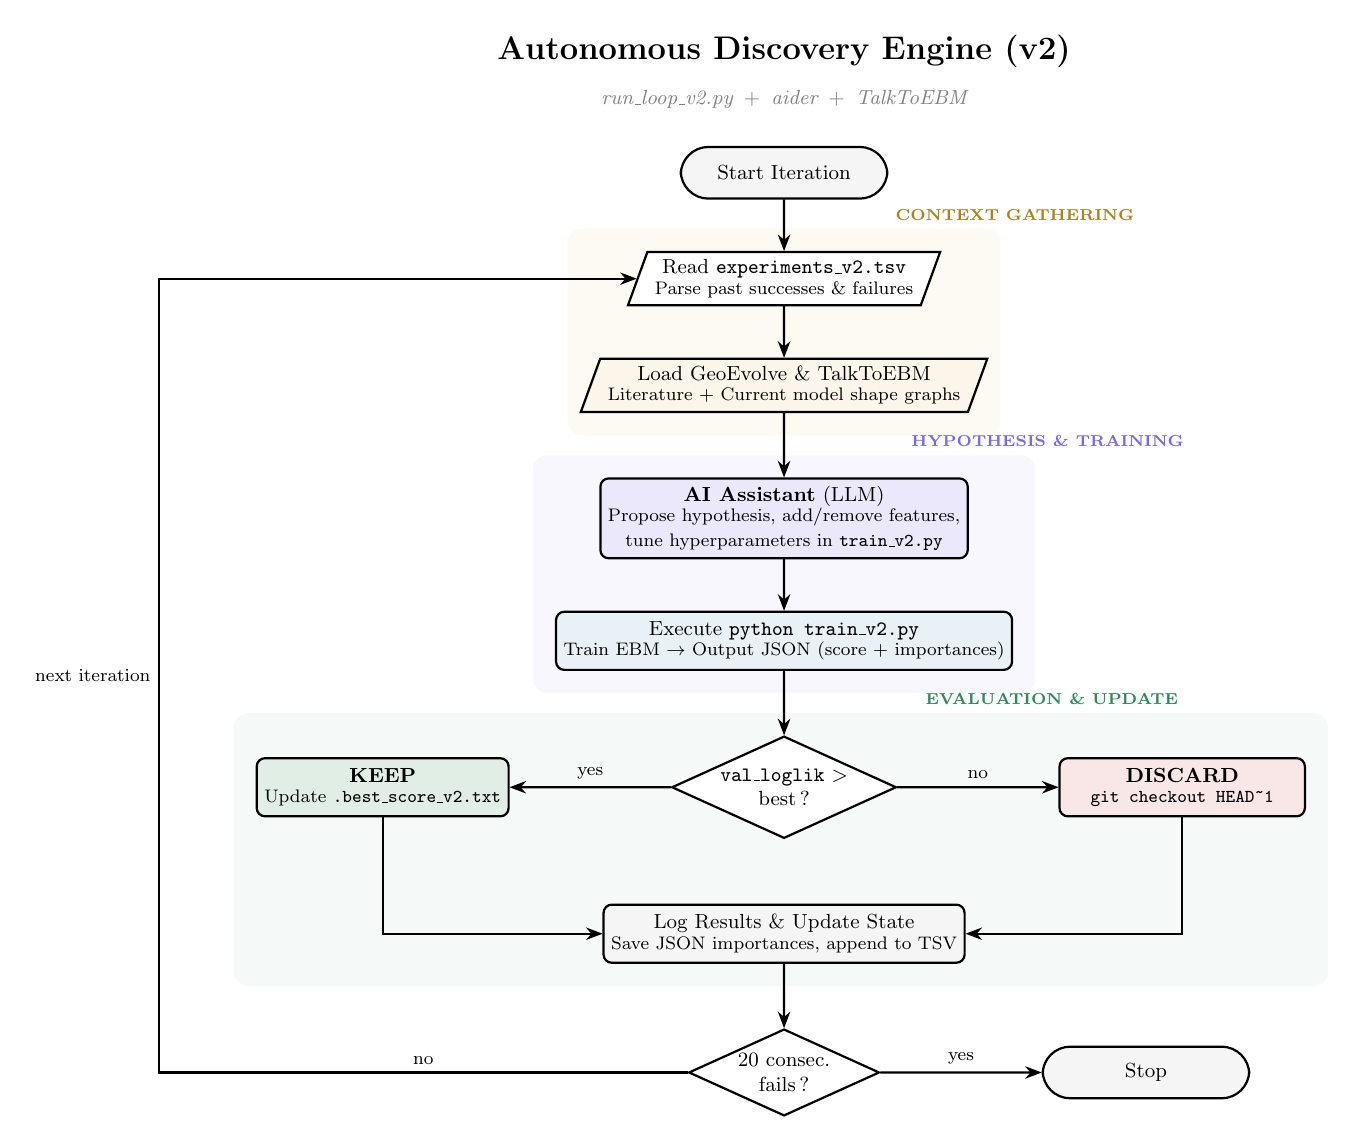
\begin{tikzpicture}[
    scale=0.82, transform shape, % Native TikZ scaling (Safe for A4)
    node distance=1.2cm and 2.5cm,
    every node/.style={font=\small, align=center},
    process/.style={
      rectangle, draw, rounded corners=3pt,
      minimum width=3.8cm, minimum height=0.9cm,
      fill=white, thick
    },
    decision/.style={
      diamond, draw, thick,
      minimum width=2.2cm, minimum height=1.2cm,
      inner sep=1pt, fill=white,
      aspect=2.2
    },
    startstop/.style={
      rectangle, draw, rounded corners=10pt,
      minimum width=3.2cm, minimum height=0.8cm,
      fill=bglight, thick
    },
    io/.style={
      trapezium, draw, thick,
      trapezium left angle=70, trapezium right angle=110,
      minimum width=3cm, minimum height=0.8cm,
      fill=white
    },
    arrow/.style={-{Stealth[length=6pt]}, thick},
    dasharrow/.style={-{Stealth[length=5pt]}, thick, dashed, gray},
  ]

  % --- Title ---
  \node[font=\Large\bfseries, anchor=south] at (0, 11.5)
    {Autonomous Discovery Engine (v2)};
  \node[font=\small\itshape, anchor=north, text=gray] at (0, 11.4)
    {run\_loop\_v2.py $\,+\,$ aider $\,+\,$ TalkToEBM};

  % --- Nodes ---
  \node[startstop] (start) at (0, 10) {Start Iteration};
  
  \node[io, below=0.8cm of start] (history)
    {Read \texttt{experiments\_v2.tsv}\\[-2pt]
     {\footnotesize Parse past successes \& failures}};
     
  \node[io, below=0.8cm of history, fill=contextgold!10] (t2ebm)
    {Load GeoEvolve \& TalkToEBM\\[-2pt]
     {\footnotesize Literature + Current model shape graphs}};

  % FIXED: The line break (\\) is safely outside the formatting braces
  \node[process, below=1cm of t2ebm, fill=llmpurple!15] (llm)
    {\textbf{AI Assistant} (LLM)\\[-2pt]
     {\footnotesize Propose hypothesis, add/remove features,}\\
     {\footnotesize tune hyperparameters in \texttt{train\_v2.py}}};
     
  \node[process, below=0.8cm of llm, fill=trainblue!12] (train)
    {Execute \texttt{python train\_v2.py}\\[-2pt]
     {\footnotesize Train EBM $\to$ Output JSON (score + importances)}};
     
  \node[decision, below=1cm of train] (improved)
    {\texttt{val\_loglik} $>$\\best\,?};

  % Keep branch (left)
  \node[process, left=2.5cm of improved, fill=keepgreen!15] (keep)
    {\textbf{KEEP}\\[-2pt]
     {\footnotesize Update \texttt{.best\_score\_v2.txt}}};
     
  % Discard branch (right)
  \node[process, right=2.5cm of improved, fill=discardred!12] (discard)
    {\textbf{DISCARD}\\[-2pt]
     {\footnotesize \texttt{git checkout HEAD\textasciitilde1}}};

  \node[process, below=1cm of improved, fill=bglight] (log)
    {Log Results \& Update State\\[-2pt]
     {\footnotesize Save JSON importances, append to TSV}};
     
  \node[decision, below=1cm of log] (stopcheck)
    {20 consec.\\fails\,?};

  \node[startstop, right=2.5cm of stopcheck] (stop) {Stop};

  % --- Safe Routing Coordinates for Loop Arrows ---
  \coordinate (rightRoute) at ($ (discard.east) + (2.2cm, 0) $);
  \coordinate (leftRoute) at ($ (keep.west) - (1.5cm, 0) $);

  % --- Arrows ---
  \draw[arrow] (start) -- (history);
  \draw[arrow] (history) -- (t2ebm);
  \draw[arrow] (t2ebm) -- (llm);
  \draw[arrow] (llm) -- (train);
  \draw[arrow] (train) -- (improved);

  \draw[arrow] (improved.west) -- node[above, font=\footnotesize] {yes} (keep.east);
  \draw[arrow] (improved.east) -- node[above, font=\footnotesize] {no} (discard.west);

  \draw[arrow] (keep.south) |- (log);
  \draw[arrow] (discard.south) |- (log);

  \draw[arrow] (log) -- (stopcheck);
  \draw[arrow] (stopcheck.east) -- node[above, font=\footnotesize] {yes} (stop.west);
  
  \draw[arrow] (stopcheck.west) -- node[above, font=\footnotesize] {no} 
    (stopcheck.west -| leftRoute) -- 
    node[left, font=\footnotesize] {next iteration} 
    (history.west -| leftRoute) -- (history.west);

  % --- Phase labels (right side) ---
  \begin{scope}[on background layer]
    \node[fit=(history)(t2ebm),
      fill=contextgold!5, rounded corners=5pt, inner sep=8pt,
      label={[font=\scriptsize\bfseries, text=contextgold!80!black]above right:CONTEXT GATHERING}] {};
    \node[fit=(llm)(train),
      fill=llmpurple!5, rounded corners=5pt, inner sep=8pt,
      label={[font=\scriptsize\bfseries, text=llmpurple]above right:HYPOTHESIS \& TRAINING}] {};
    \node[fit=(improved)(keep)(discard)(log),
      fill=keepgreen!5, rounded corners=5pt, inner sep=8pt,
      label={[font=\scriptsize\bfseries, text=keepgreen]above right:EVALUATION \& UPDATE}] {};
  \end{scope}
\end{tikzpicture}
\end{center}
\vspace*{\fill}

\end{document}